%%%%%%%%%%%%%%%%%%%%%%%%%%%%%%%%%%%%%%%%%
% a0poster Landscape Poster
% LaTeX Template
% Version 1.0 (22/06/13)
%
% The a0poster class was created by:
% Gerlinde Kettl and Matthias Weiser (tex@kettl.de)
% 
% This template has been downloaded from:
% http://www.LaTeXTemplates.com
%
% License:
% CC BY-NC-SA 3.0 (http://creativecommons.org/licenses/by-nc-sa/3.0/)
%
%%%%%%%%%%%%%%%%%%%%%%%%%%%%%%%%%%%%%%%%%

%----------------------------------------------------------------------------------------
%	PACKAGES AND OTHER DOCUMENT CONFIGURATIONS
%----------------------------------------------------------------------------------------

\documentclass[a0,landscape]{a0poster}

\usepackage{multicol} % This is so we can have multiple columns of text side-by-side
\columnsep=100pt % This is the amount of white space between the columns in the poster
\columnseprule=3pt % This is the thickness of the black line between the columns in the poster

\usepackage[svgnames]{xcolor} % Specify colors by their 'svgnames', for a full list of all colors available see here: http://www.latextemplates.com/svgnames-colors

\usepackage{times} % Use the times font
%\usepackage{palatino} % Uncomment to use the Palatino font

\usepackage{subcaption} %  for subfigures environments 
\usepackage{graphicx} % Required for including images
\graphicspath{{figures/}} % Location of the graphics files
\usepackage{booktabs} % Top and bottom rules for table
\usepackage[font=small,labelfont=bf]{caption} % Required for specifying captions to tables and figures
\usepackage{amsfonts, amsmath, amsthm, amssymb} % For math fonts, symbols and environments
\usepackage{wrapfig} % Allows wrapping text around tables and figures

\begin{document}

%----------------------------------------------------------------------------------------
%	POSTER HEADER 
%----------------------------------------------------------------------------------------

% The header is divided into three boxes:
% The first is 55% wide and houses the title, subtitle, names and university/organization
% The second is 25% wide and houses contact information
% The third is 19% wide and houses a logo for your university/organization or a photo of you
% The widths of these boxes can be easily edited to accommodate your content as you see fit

\begin{minipage}[b]{0.55\linewidth}
\veryHuge \color{NavyBlue} \textbf{Attentive Sequence-to-Sequence Learning for \\
  Diacritic Restoration of Yor{\`u}b{\'a} Language Text} \color{Black}\\ % Title
  
\huge \textbf{Iroro Fred \d{\`O}n\d{\`o}m\d{\`e} Orife}\\ % Author(s)
\huge Niger-Volta Language Technologies Institute\\ % University/organization
\end{minipage}
%
\begin{minipage}[b]{0.25\linewidth}

\includegraphics[width=1cm]{logo.png} % Logo or a photo of you, adjust its dimensions here
\end{minipage}
%
\begin{minipage}[b]{0.25\linewidth}
\color{DarkSlateGray}\Large \textbf{Contact Information:}\\
\texttt{github.com/niger-volta-LTI} \\
\texttt{iroro@alumni.cmu.edu}\\ % Email address
\end{minipage}
%
%\begin{minipage}[b]{0.25\linewidth}
%
\includegraphics[width=15cm]{logo.png} % Logo or a photo of you, adjust its dimensions here
%\end{minipage}

\vspace{1cm} % A bit of extra whitespace between the header and poster content

%----------------------------------------------------------------------------------------

\begin{multicols}{4} % This is how many columns your poster will be broken into, a poster with many figures may benefit from less columns whereas a text-heavy poster benefits from more

%----------------------------------------------------------------------------------------
%	ABSTRACT
%----------------------------------------------------------------------------------------

\color{Navy} % Navy color for the abstract

\begin{abstract}

Yor{\`u}b{\'a} is a widely spoken West African language with a writing system rich in tonal and orthographic diacritics. With very few exceptions, diacritics are omitted from electronic texts, due to limited device and application support. Diacritics provide morphological information, are crucial for lexical disambiguation, pronunciation and are vital for any Yor{\`u}b{\'a} text-to-speech (TTS), automatic speech recognition (ASR) and natural language processing (NLP) tasks. Reframing Automatic Diacritic Restoration (ADR) as a machine translation task, we experiment with two different attentive Sequence-to-Sequence neural models to process undiacritized text. On our evaluation dataset, this approach produces diacritization error rates of less than 5\%. We have released pre-trained models, datasets and source-code as an open-source project to advance efforts on Yor{\`u}b{\'a} language technology.

\end{abstract}

%----------------------------------------------------------------------------------------
%	INTRODUCTION
%----------------------------------------------------------------------------------------

\color{SaddleBrown} % SaddleBrown color for the introduction

\section*{Introduction}

Yor{\`u}b{\'a} is a tonal language spoken by more than 40 Million people in the countries of Nigeria, Benin and Togo in West Africa. There are an additional million speakers in the African diaspora, making it the most broadly spoken African language outside Africa. 

On modern computing platforms, the vast majority of Yor{\`u}b{\'a} text is written in plain ASCII, without diacritics. This presents grave problems for usage of the standard orthography via electronic media, which has implications for the unambiguous pronunciation of Yor{\`u}b{\'a}'s lexical and grammatical tones by both human speakers and TTS systems. Improper handling of diacritics also degrades the performance of document retrieval via search engines and frustrates every kind of Natural Language Processing (NLP) task, notably machine translation to and from Yor{\`u}b{\'a}. Finally, correct diacritics are mandatory in reference transcripts for any Automatic Speech Recognition (ASR) task.

\begin{enumerate}
\item We propose two different NMT approaches, using soft-attention and self-attention sequence-to-sequence (seq2seq) models \cite{bahdanau2014neural, vaswani2017attention}, to rectify undiacritized Yor{\`u}b{\'a} text.
\item Datasets, pre-trained models and source code are an open-source project at \textbf{\texttt{github.com/niger-volta-LTI/yoruba-adr}}
\end{enumerate}

\color{DarkSlateGray} % DarkSlateGray color for the rest of the content

%----------------------------------------------------------------------------------------
%	MATERIALS AND METHODS
%----------------------------------------------------------------------------------------

\section*{Ambiguity in Undiacritized Yor{\`u}b{\'a} text }

Automatic Diacritic Restoration (ADR), which goes by other names such as Unicodification or deASCIIfication is a process which attempts to resolve the ambiguity present in undiacritized text. Undiacritized Yor{\`u}b{\'a} text has a high degree of ambiguity. Adegbola et al. state that for ADR the ``prevailing error factor is the number of valid alternative arrangements of the diacritical marks that can be applied to the vowels and syllabic nasals within the words".

For our training corpus of 1M words, we quantify the ambiguity by the percentage of all words that have diacritics, 85\%; the percentage of unique non-diacritized word types that have two or more diacritized forms, 32\%, and the lexical diffusion or \emph{LexDif} metric, which conveys the average number of alternatives for each non-diacritized word, 1.47. 

\begin{center}\vspace{1cm}
  \begin{tabular}{lcl}
    \toprule
    \multicolumn{2}{c}{\textbf{Characters}} & \textbf{Examples}  \\
    \midrule
    {\`a} {\'a} \v{a} & \textbf{a} & gb{\`a} \emph{(spread)}, gba \emph{(accept)}, gb{\'a} \emph{(hit)}    \\  
    {\`e} {\'e} \d{e} \d{\`e} \d{\'e} & \textbf{e} & es{\'e} \emph{(cat)}, {\`e}s{\`e} \emph{(dye)}, \d{e}s\d{\`e} \emph{(foot)} \\
    {\`i} {\'i} & \textbf{i} & {\`i}l{\'u} \emph{(town)}, ilu \emph{(opener)}, {\`i}l{\`u} \emph{(drum)}\\  
    {\`o} {\'o} \d{o} \d{\`o} \d{\'o} \v{o} & \textbf{o} & \d{o}k\d{\'o} \emph{(hoe)}, \d{\`o}k\d{\`o} \emph{(spear)}, \d{o}k\d{\`o} \emph{(vehicle)}\\  
    {\`u} {\'u} \v{u} & \textbf{u} & mu \emph{(drink)}, m{\`u} \emph{(sink)},  m{\'u} \emph{(sharp)} \\
    \midrule
    {\`n} {\'n} \={n} & \textbf{n} & {n} \emph{(I)}, {\'n} (continuous aspect marker) \\  
    \d{s} & \textbf{s} &  {s}{\'a} \emph{(run)}, \d{s}{\'a} \emph{(fade)}, \d{s}{\`a} \emph{(choose)} \\  
    \bottomrule
  \end{tabular}
\captionof{table}{Diacritized forms for each non-diacritic character}
\end{center}\vspace{1cm}

Further, 64\% of all unique, non-diacritized monosyllabic words possess multiple diacritized forms. When we consider the distribution of ambiguity over grammatical function, we recognize the added difficulty of tasks like the lexical disambiguation of non-diacritized Yor{\`u}b{\'a} verbs, which are predominantly monosyllabic.
\\
Finally, there are tonal changes, which are rules about how tonal diacritics on a specific word are \emph{altered} based on context. 
\begin{center}\vspace{1cm}
\begin{tabular}{clll}
   \toprule
   \textbf{Verb}  & \textbf{Phrase} & \textbf{Translation}  & \textbf{Tone}\\
   \midrule
   t{\`a}  & o t{\`a} a & he sells it & Low \\ 
                    & o ta i\d{s}u, o ta\d{s}u & he sells yams & Mid\\  
   \midrule
    t{\`a} & o ta {\`i}w{\'e} & he sells books & Mid \\ 
                    & o t{\`a}w{\'e} & he sells books & Low\\  
   \bottomrule
 \end{tabular}
\captionof{table}{Tonal Changes}
\end{center}

%------------------------------------------------

\section*{A Sequence-to-Sequence Approach}

Expressing ADR as a machine translation problem, we treat undiacritized text and diacritized text as source and target languages respectively in a NMT formulation. We experimented two different NMT approaches:

\begin{enumerate}
\item \textbf{Soft-attention} based on the work of Bahdanau et al. \cite{bahdanau2014neural}, extends the RNN-Encoder-Decoder design with an attention mechanism that allows the decoder to observe different source words for each target word.
\item \textbf{Self-attention} aims to improve on limitations of RNNs, i.e. high computational complexity and non-parallelizeable computation. For both the encoder and decoder, the Transformer model, proposed by Vaswani et al. \cite{vaswani2017attention}, employs stacks of self-attention layers in lieu of RNNs.
\end{enumerate}

%----------------------------------------------------------------------------------------
%	RESULTS 
%----------------------------------------------------------------------------------------

\section*{Experiments \& Results}

We obtained a very small but fully diacritized text from the Lagos-NWU conversational speech corpus by Niekerk, et. al. We also created our own medium-sized corpus by web-crawling the two Yor{\`u}b{\'a}-language websites.

\begin{center}
  \begin{tabular}{lll}
    \toprule
    \textbf{\# words} & \textbf{Source URL}  & \textbf{Description} \\
    \midrule
    24,868 & rma.nwu.ac.za  & Lagos-NWU corpus \\  
    50,202 & theyorubablog.com & language blog\\  
    910,401 & bible.com & online bible webite \\
    \bottomrule
  \end{tabular}
  \captionof{table}{Training data subsets}
\end{center}

To better understand the dataset split, we computed a perplexity of 575.6 for the test targets with a language model trained over the training targets. The \{source, target\} vocabularies for training and test sets have \{11857, 18979\} and \{4042, 5641\} word types respectively.

We built the soft-attention and self-attention models with the Python 3 implementation of OpenNMT, an open-source toolkit created by the Klein et al. Our training hardware configuration was a standard AWS EC2 p2.xlarge instance with a NVIDIA K80 GPU, 4 vCPUs and 61GB RAM. 

\begin{center}
  \begin{tabular}{ccccc}
    \toprule
    \textbf{Attention} & \textbf{Size} & \textbf{RNN} & \textbf{Train\%} & \textbf{Test\%}\\
    \midrule
    soft + dot & 2L 512 & LSTM & 96.2 & 90.1  \\
    soft + add & 2L 512 & LSTM & 95.9 & 90.1  \\
	soft + tanh & 2L 512 & GRU & 96.2 & 89.7  \\ 
	soft + tanh & 1L 512 & GRU  & 97.8 & 89.7  \\ 
	\midrule
    self & 6L 512   & -  & 98.5 & 95.4 \\
    \bottomrule
  \end{tabular}
  \captionof{table}{Results}
\end{center}

The verbs \textbf{b{\`a}j\d{\'e}} (to spoil), or \textbf{j{\`u}l\d{o}} (to be more than) are discontinuous morphemes, or splitting verbs. In Table 5, the first example shows the model has learnt the diacritics necessary for \textbf{l\d{o}} following a previously predicted \textbf{j{\`u}}. In the second example, we note the ambiguity of the three occurrences of the undiacritized \textbf{si}, with two diacritized forms, \textbf{s{\`i}}, \textbf{s{\'i}}. An examination of the attention weight matrix for this example revealed that the third instance \textbf{s{\'i}} attends to the previous \textbf{s{\'i}} and that the first two attend to each other.

\begin{center}
  \begin{tabular}{rl}
    \toprule
    \textbf{source}  & emi ni oye ju awon agba lo nitori mo gba eko re\\
    \textbf{target} & {\`e}mi ni {\`o}ye j{\`u} {\`a}w\d{o}n {\`a}gb{\`a} l\d{o} n{\'i}tor{\'i} mo gba \d{\`e}k\d{\'o} r\d{e} \\
    \textbf{prediction} & {\`e}mi ni {\`o}ye \underline{\textbf{j{\`u}} {\`a}w\d{o}n {\`a}gb{\`a} \textbf{l\d{o}}} n{\'i}tor{\'i} mo gba \d{\`e}k\d{\'o} r\d{e}\\
    \midrule
    \textbf{source} & emi yoo si si oju mi si juda \\
    \textbf{target} & {\`e}mi y{\'o}{\`o} s{\`i} s{\'i} oj{\'u} mi s{\'i} il{\'e} j{\'u}d{\`a} \\
    \textbf{prediction} & {\`e}mi y{\'o}{\`o} s{\`i} s{\'i} oj{\'u} mi s{\'i} il{\'e} j{\'u}d{\`a} \\
    \midrule
	\textbf{source}  & oun ko si ni ko ile ini re sile \\
	\textbf{target} &   {\`o}un k{\`o} s{\`i} n{\'i} \textbf{k\d{o}} il\d{\`e} {\`i}n{\'i}  r\d{\`e} s{\'i}l\d{\`e}\\
	\textbf{prediction} &  {\`o}un k{\`o} s{\`i} n{\'i} \textbf{k\d{\'o}} il\d{\`e} {\`i}n{\'i}  r\d{\`e} s{\'i}l\d{\`e} \\ 
    \bottomrule
  \end{tabular}
  \captionof{table}{Example predictions}
\end{center}

\begin{center}
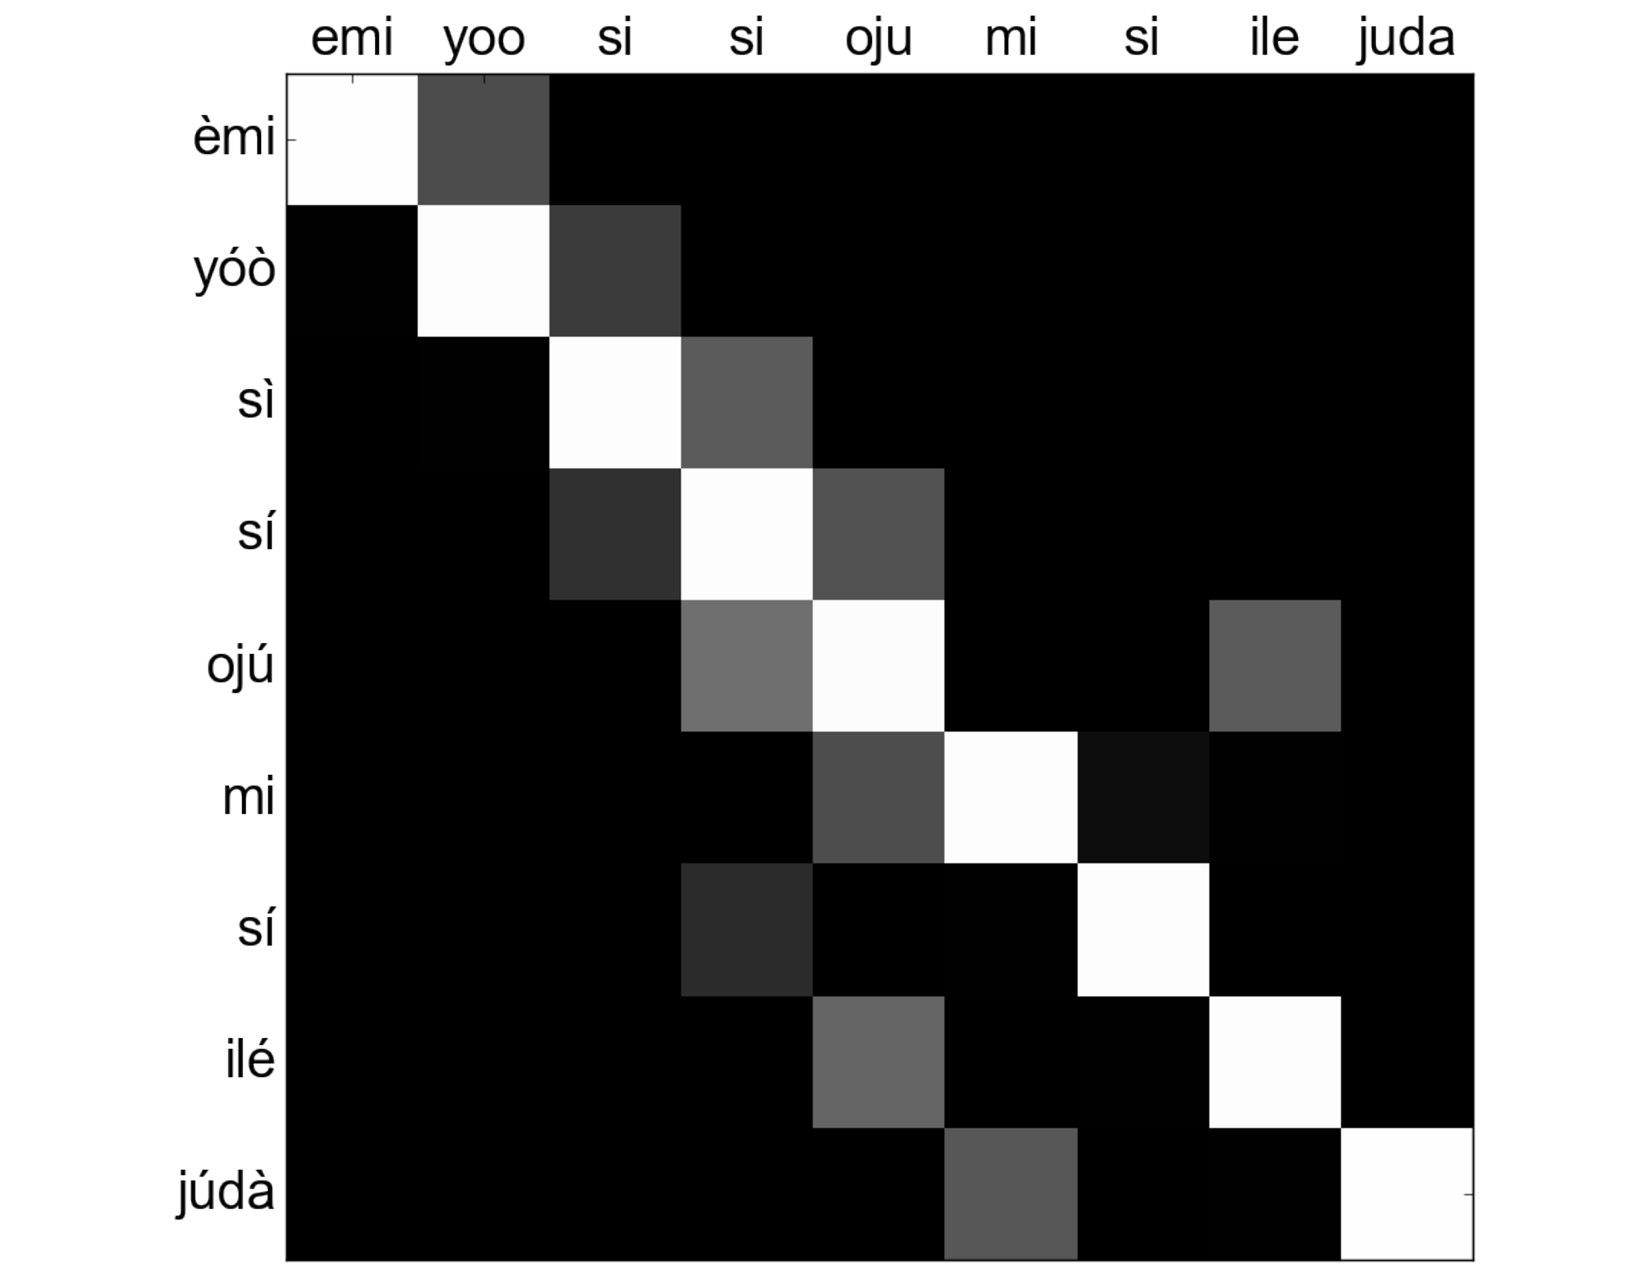
\includegraphics[width=0.55\linewidth]{emi_yoo_AttentionWeights}
\end{center}
\begin{center}
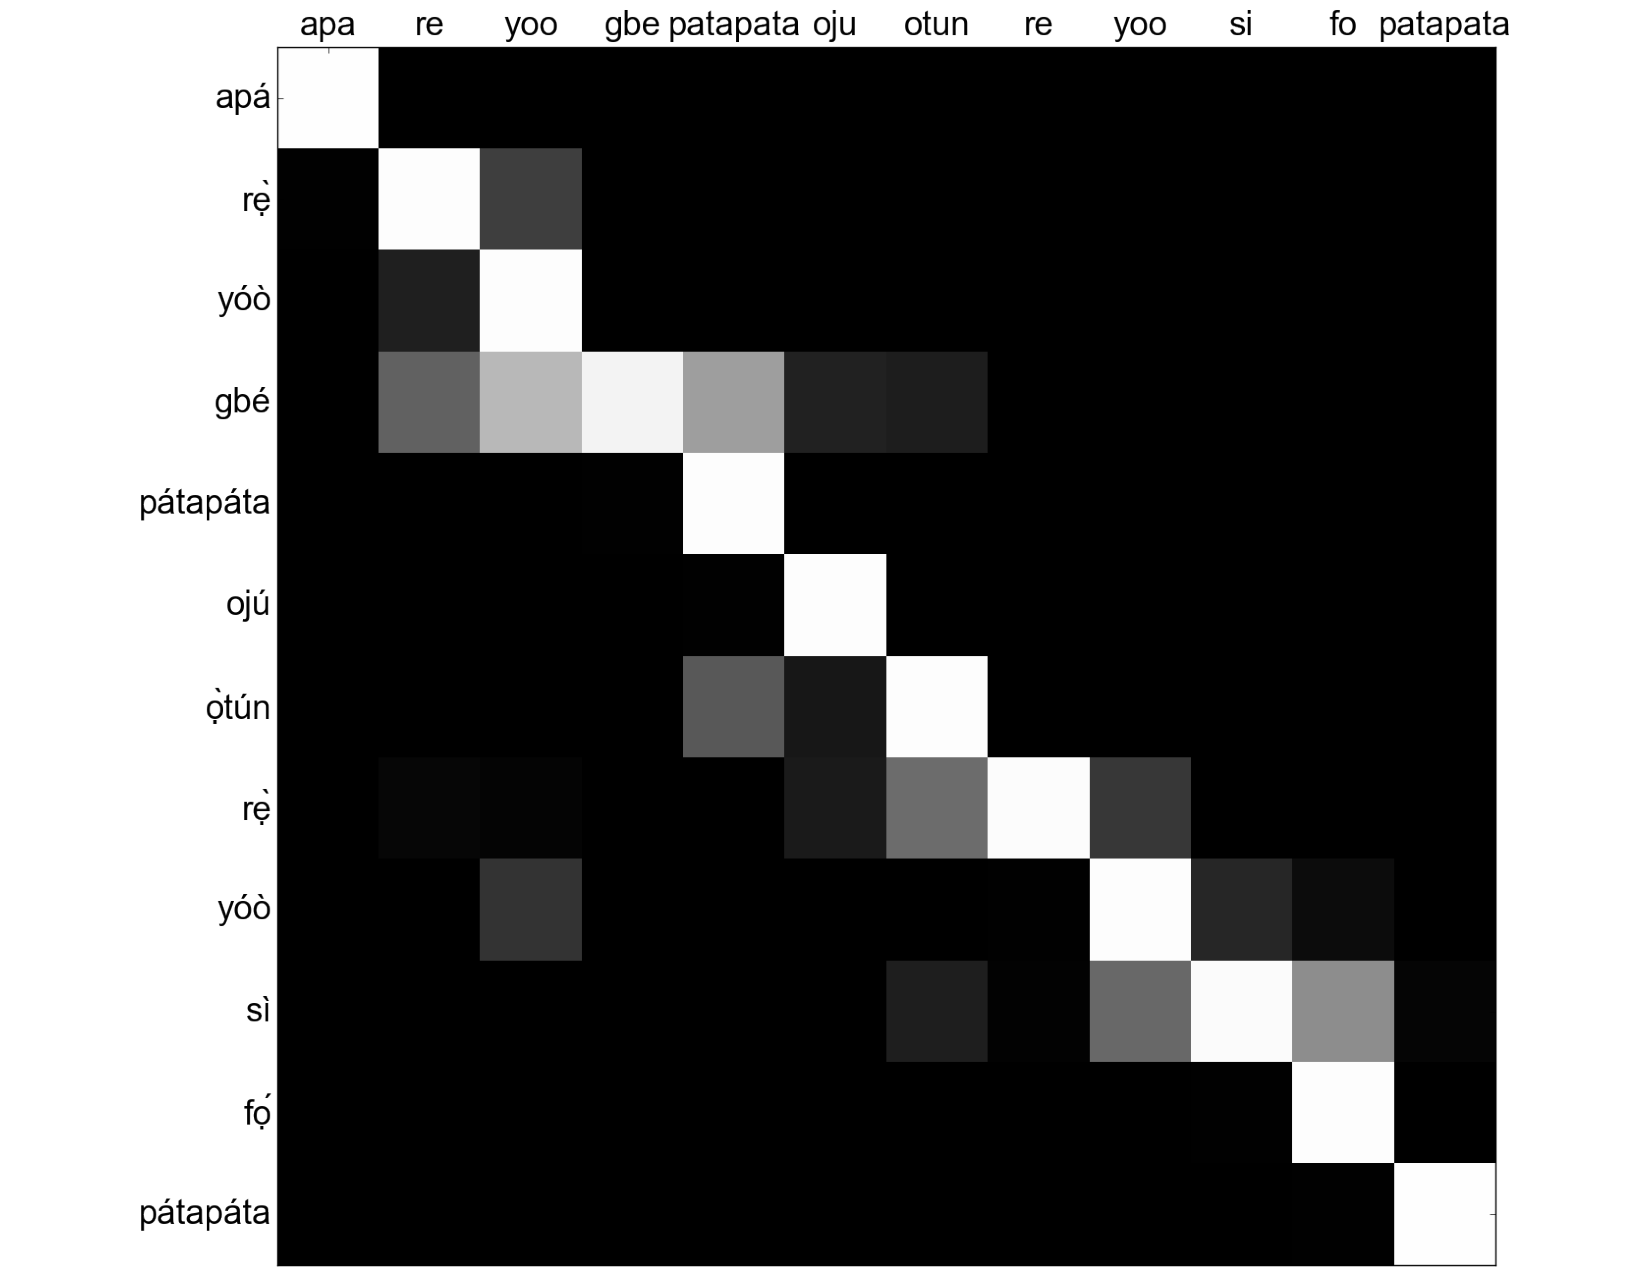
\includegraphics[width=0.65\linewidth]{patapata_AttentionWeights}
\captionof{figure}{Attention Weights}
\end{center}

%----------------------------------------------------------------------------------------
%	CONCLUSIONS
%----------------------------------------------------------------------------------------

\color{SaddleBrown} % SaddleBrown color for the conclusions to make them stand out

\section*{Conclusions}

\begin{itemize}
\item Attention-based sequence-to-sequence learning approaches perform well on the Yor{\`u}b{\'a} diacritic restoration task.
\item Our approach minimizes the manual work needed to quickly create a high quality text corpus for TTS and MT tasks.
\item To make ADR more suitable as a preprocessing step for end-user text processing applications or any business usage, it will be necessary to augment training the corpus with more general purpose text.
\end{itemize}

\color{DarkSlateGray} % Set the color back to DarkSlateGray for the rest of the content

%----------------------------------------------------------------------------------------
%	FORTHCOMING RESEARCH
%----------------------------------------------------------------------------------------

\section*{Forthcoming Research}

Avenues for future work include evaluating previous approaches to Yor{\`u}b{\'a} ADR on the present dataset, growing the training corpus and training superior word embeddings. We see the application of ADR to OCR output of scanned books as a fruitful next step in building high quality text corpora.

%----------------------------------------------------------------------------------------
%	REFERENCES
%----------------------------------------------------------------------------------------

\nocite{*} % Print all references regardless of whether they were cited in the poster or not
\bibliographystyle{plain} % Plain referencing style
\bibliography{sample} % Use the example bibliography file sample.bib


%----------------------------------------------------------------------------------------

\end{multicols}
\end{document}